% Virtual Environment for Individual-Based Modeling - Part II
%
% Advanced Project II - Jacobs University Bremen
% Supervisor: Dr. Stefan Kettemann
%
% Created on January 10, 2019
%
% Authors:
%   Ralph Florent <r.florent@jacobs-university.de>
%   Davi Tavares <davi.tavares@leibniz-zmt.de>
%   Agostino Merico <a.merico@jacobs-university.de>

% ==============================================================================
% START: Overview of VE-IBM Part I
% ==============================================================================

\section{Overview}
The goal of the first part of the \emph{Virtual Environment for Individual-Based Modeling} project was clear and simple: create a virtual environment prototype while using an ABM technique to study the habitat use by waterbirds in coastal lagoons of the tropics. Therefore, we built our assumptions on the general model concept shown below in Figure \ref{fig:concept-1v}.

As the second part of the project is built upon this first part, we retake some points that are relatively important and constitute the core element of the second release. In the section, we give an overview of the past work and discuss the correlation between both the first and second version.

\begin{figure}[!ht]
    \centering
    \frame{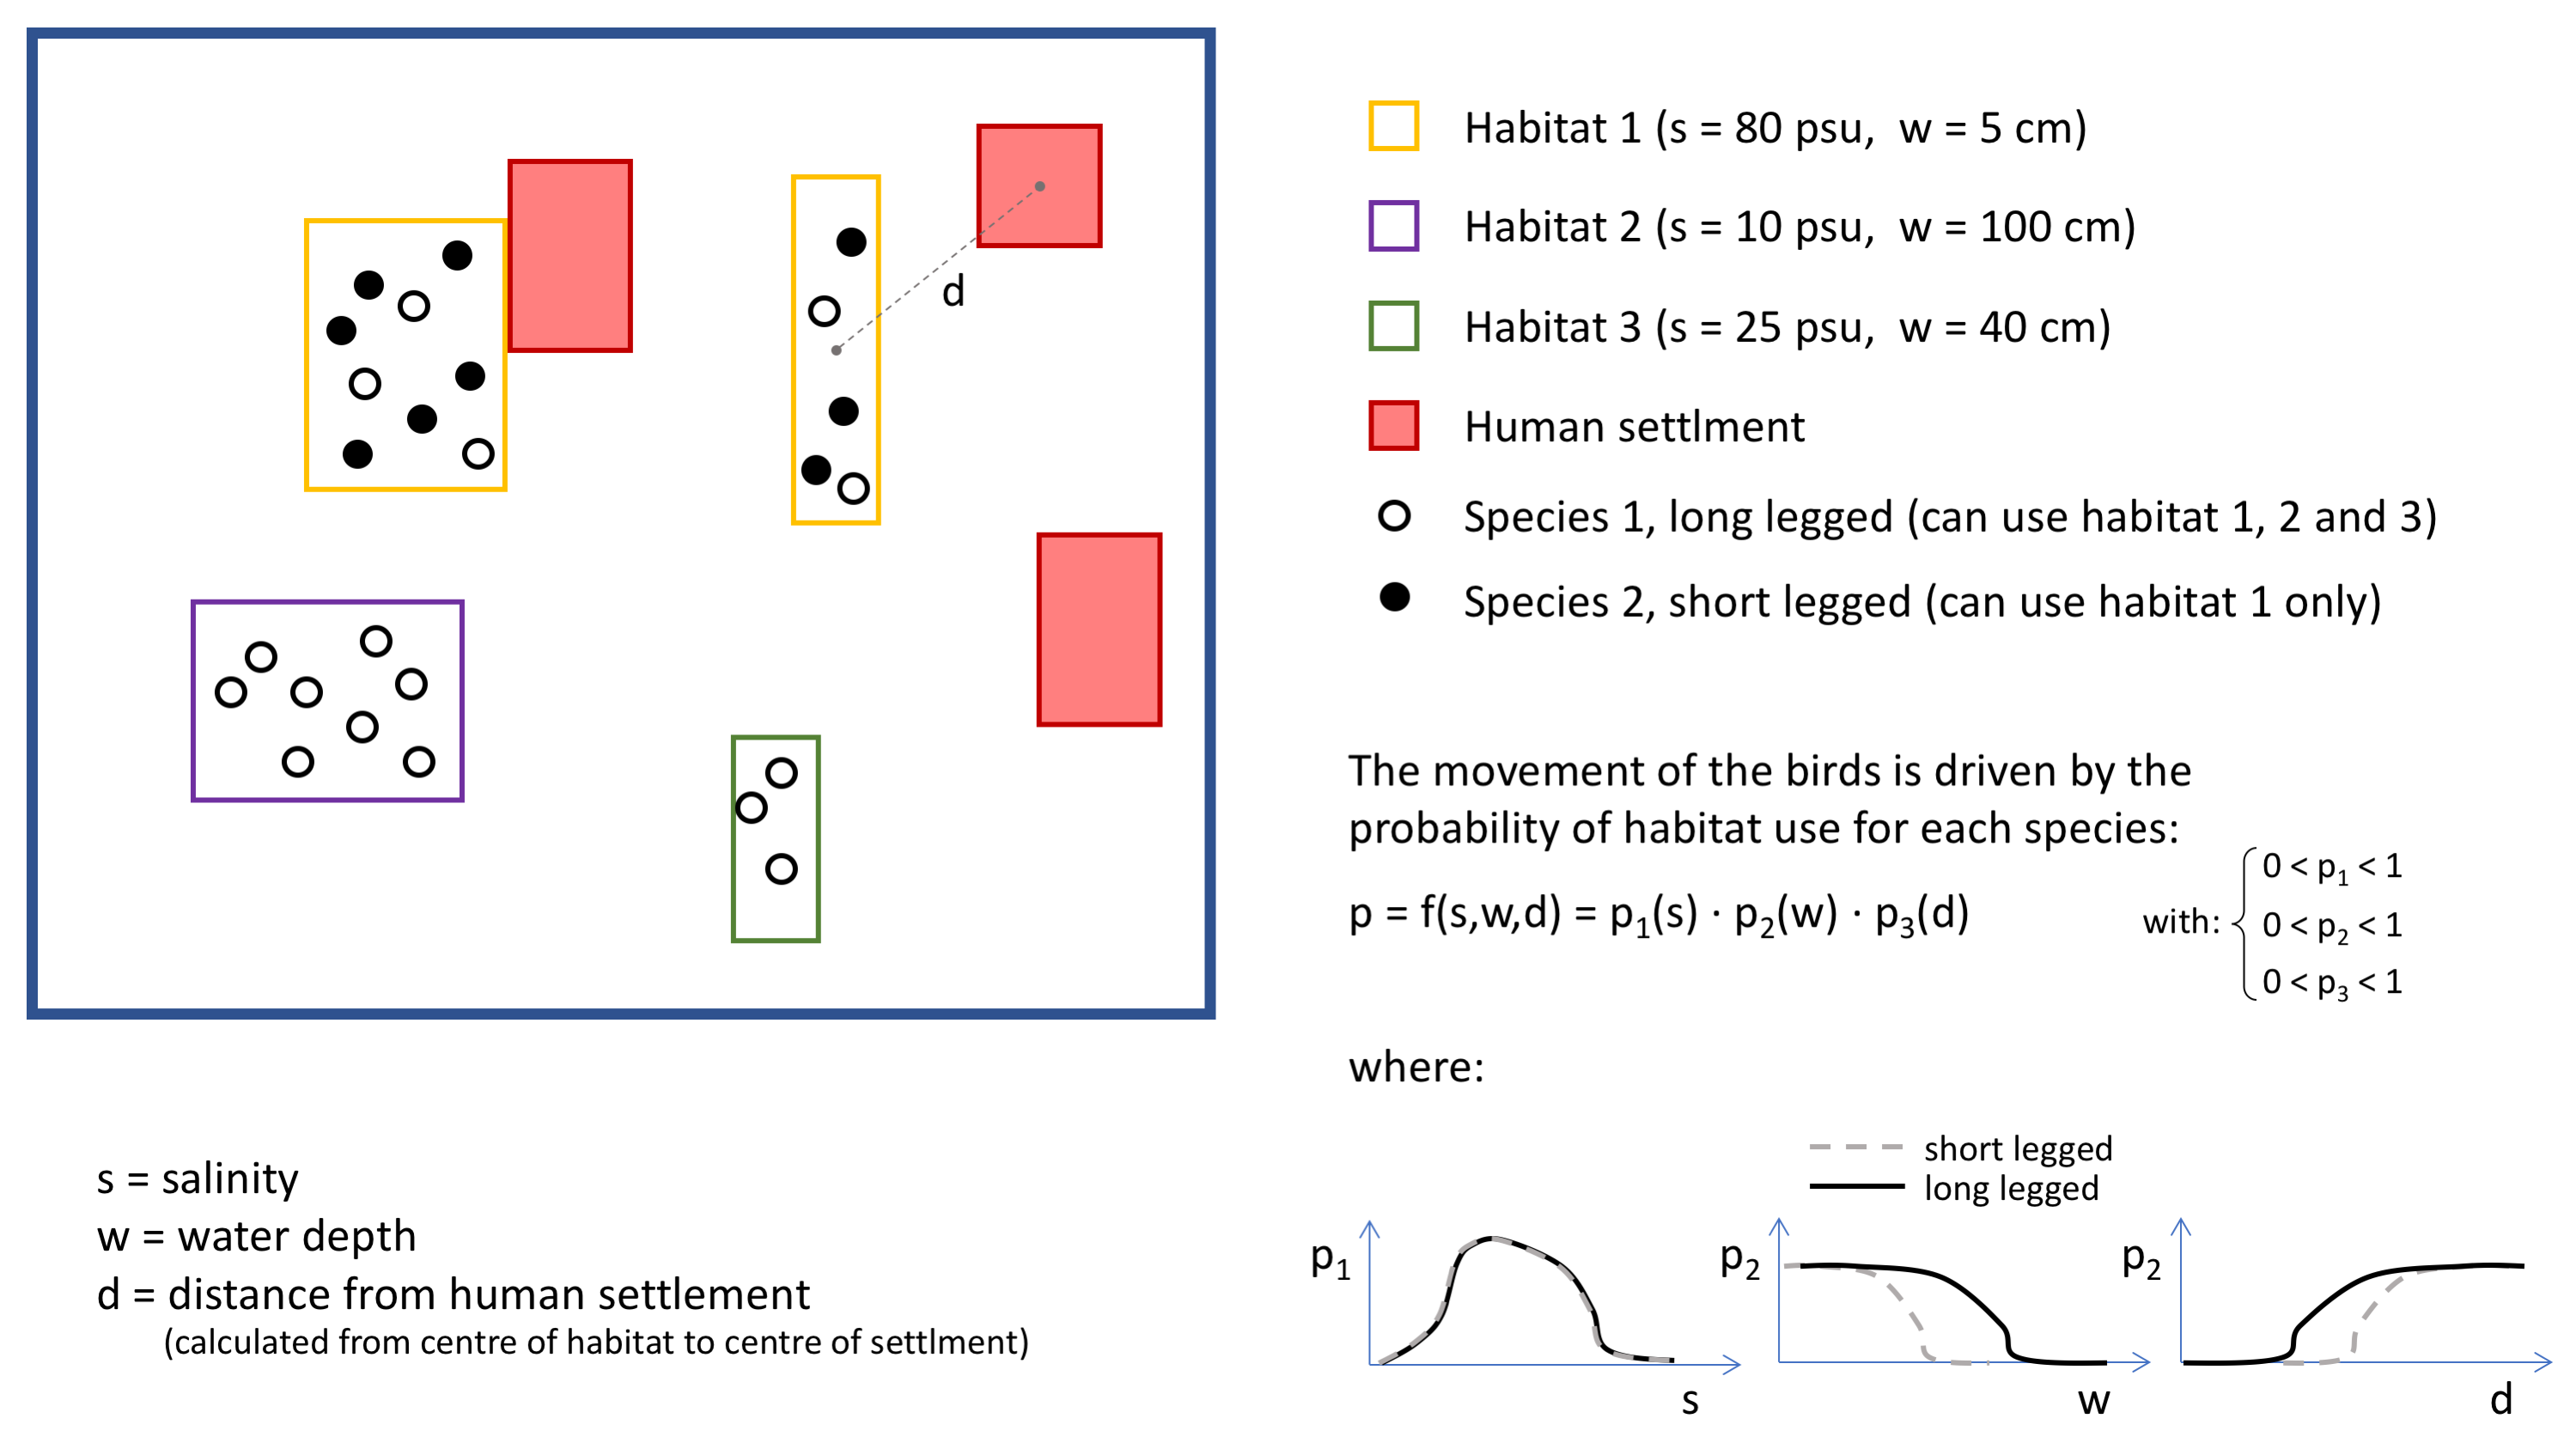
\includegraphics[scale=0.33]{docs/concept_1v.png}}
    \caption{Model concept for the \emph{Virtual Environment for Indivual-Based Modeling - Part I}.}
    \label{fig:concept-1v}
\end{figure}

\subsection{Theory review}
In the first part of the project, some core elements or components such as  \emph{warterbirds} and \emph{lagoons} of the system are discussed and, subsequently, their digital representation within the prototype based on the assumptions derived from previous investigations.

Recalling that tropical coastal lagoons are shallow aquatic ecosystems located at the boundary between terrestrial and marine environments \cite{tavares2015environmental}, the high environmental heterogeneity of coastal lagoons, in both temporal and spatial scales, provides habitats for aquatic bird species with different ecological needs \cite{ntiamoa1998water, paracuellos2004factors, tavares2013inventory}. Seven environmental variables mainly characterize these habitats and water depth is the most important variable influencing the waterbird assemblage \cite{tavares2015environmental}.

On the other hand, the aquatic birds or \emph{waterbirds} inhabiting the coastal lagoons were, according to a survey conducted by Tavares D.C. et al. in 2015 \cite{tavares2015environmental}, grouped into guilds\footnote{ Blondel proposed the guild concept in 2003 \cite{blondel2003guilds}.} reflecting species' foraging habits and morphology. The six identified guilds were: diving birds (grebes), dabbling ducks (belonging to the genera Dendrocygna and Anas), large wading birds (herons, egrets, and storks), vegetation gleaners (jacanas and gallinules), fishing birds (gulls and terns) and small wading birds \cite{tavares2014variaccao}.

Agent-Based Modeling is a computational simulation framework based on intense processing and algorithmic calculations due to the fact the typical context in which the ABM is used is to study the collective behavior of a large number of components or agents \cite{rflorent2019veibm1}.

\subsection{Methods}
The core functionality of the project is based on a programmatically-implemented coding procedure that allows to explore certain programming techniques and choose the most convenient workflow for building the first VE prototype.

Its workflow scheme (as illustrated in Figure \ref{fig:workflow-scheme}), includes some internal processes that were based on the following premises: \emph{Initialize, Observe}, and \emph{Update}, where:
\begin{enumerate}
    \item \textit{Initialize}: stands for initial conditions of the system
    \item \textit{Observe}: displays a snaphot of the current state of the system
    \item \textit{Update}: generates a new state of the system by computing some random movements of the agents (based on specific factors).
\end{enumerate}

\begin{figure}[!ht]
    \centering
    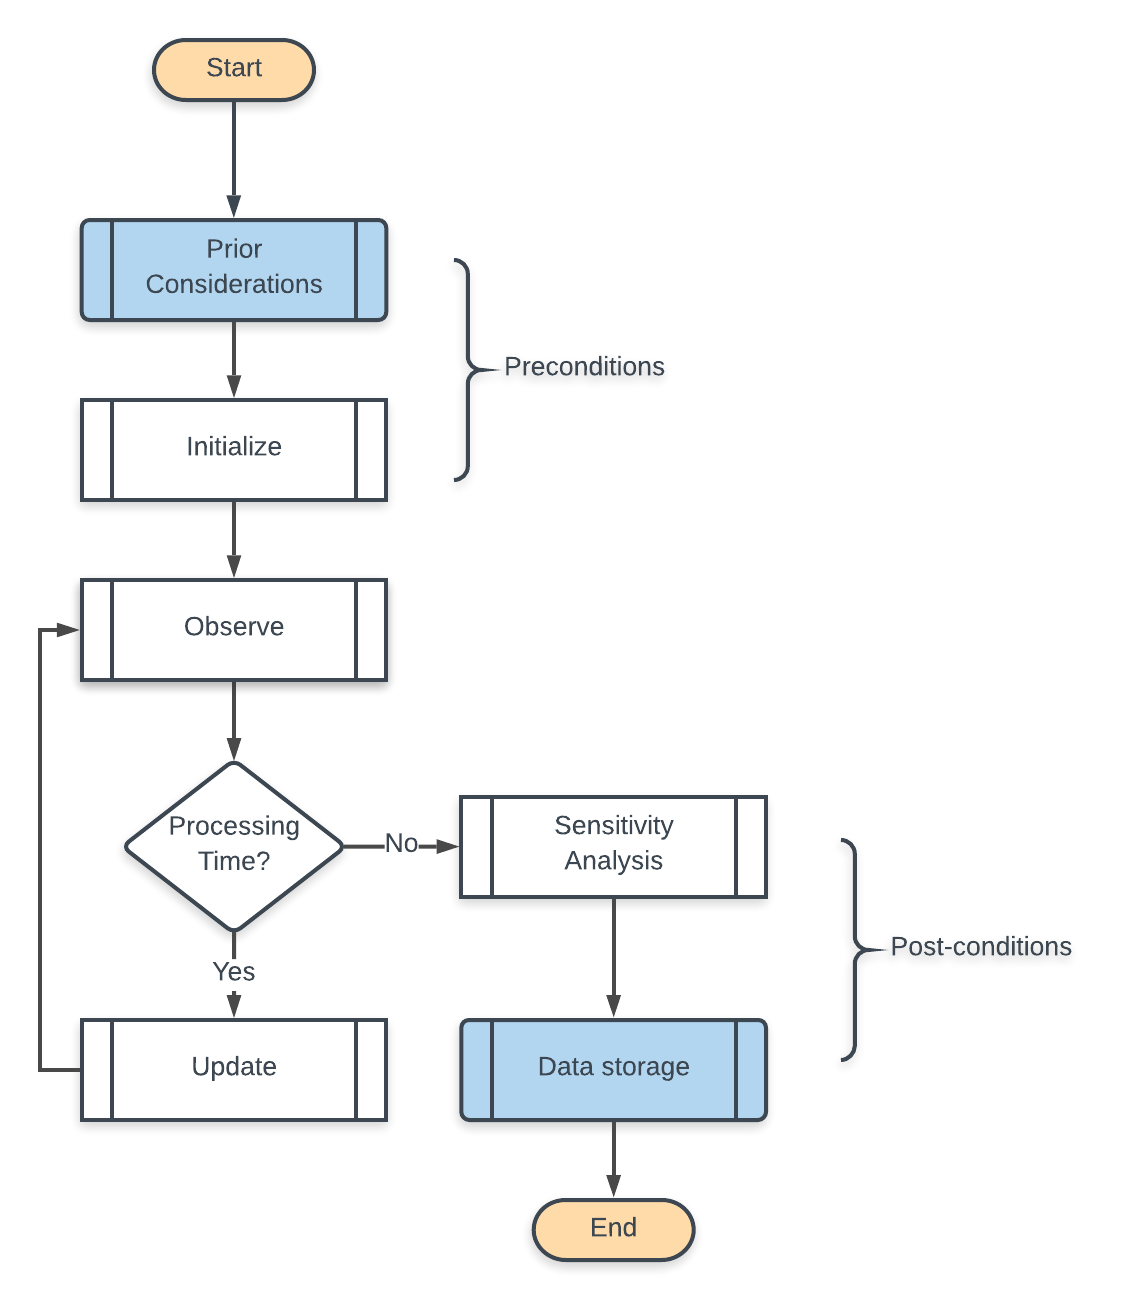
\includegraphics[scale=0.33]{docs/workflow-scheme.png}
    \caption{Workflow diagram \\ (credits: made with \emph{Lucidchart})}
    \label{fig:workflow-scheme}
\end{figure}

The VE prototype was essentially a digital representation of an ABM system where each component of that system relies on the interaction and interconnection with other involved elements in an organized flow. The diagram in Figure \ref{fig:workflow-scheme} was used as a visual aid expressing the intended performing flow of the components within the system.

\subsection{Results}
After conducting successfully two (2) pilot tests, we combined them to shape a final prototype that represents the model concept illustrated in Figure \ref{fig:concept-1v}.

Although this version of the VE simulation only considers certain factors that would interpret much closer to the waterbirds' lifestyle inhabiting the coastal lagoons of the tropics, yet the results were fairly satisfying. Let us retake some key notions (terms and concepts) used to ease up the interpretations of those results.
\begin{itemize}
    \item \textbf{Habitat}: a patch-focused drawing representation of the lagoons, rectangularly shaped and based on additional design settings.
    \item \textbf{Agent}: categorized as \emph{short-legged} or \emph{long-legged}, a drawing representation of the waterbirds.
\end{itemize}

It should be recalled that each run of the main script (available in Appendix \ref{sec:code-repo}) would generate different results since we did not handle a seed-oriented initial state (see Table \ref{table:ve-init}) for the components.

\begin{table}[!ht]
    \begin{center}
        \begin{tabular}{ ||l|l|| }
            \hline
            \multicolumn{2}{ ||c|| }{ \textbf{Initial Conditions}} \\
            \hline \hline % Table body (row-wise contents)
            \textbf{\textit{Total of long-legged waterbirds}} &  20 \\
            \hline
            \textbf{\textit{Total of short-legged waterbirds}} &  20 \\
            \hline
            \textbf{\textit{Processing times}} &  100 \\
            \hline
            \textbf{\textit{Threshold for }} &  $1 * e^{-7}$ \\
            \hline
            \textbf{\textit{Areas for short-legged waterbirds}} &  \texttt{one} \\
            \hline
            \textbf{\textit{Areas for long-legged waterbirds}} &  \texttt{one, two, three} \\
            \hline
            \textbf{\textit{Habitat one (big)}} & s = 80psu, w = 5cm, f = 0.3  \\
            \hline
            \textbf{\textit{Habitat one (small)}} & s = 80psu, w = 5cm, f = 2.56  \\
            \hline
            \textbf{\textit{Habitat two}} & s = 10psu, w = 5cm, f = 6.41  \\
            \hline
            \textbf{\textit{Habitat three}} & s = 25psu, w = 40cm, f = 11.53  \\
            \hline
        \end{tabular}
        \caption{Default values and parameters for the VE prototype's initial conditions.}
        \label{table:ve-init}
    \end{center}
\end{table}

As we do not intend to describe every detail of the results here, please refer the documentation of the first version (see Appendix \ref{sec:code-repo}) for further explanation.

\subsection{Outlook}
Note that in our previous work running the script would only generate a single-point dataset for each PDF over time. That is because at that time we did not consider a one-unit time processing where an \emph{update} action would be performed on every agent. Meanwhile, we discussed in the analysis of the results how to achieve a data set by tuning the habitats' characteristics and other influent factors over time. For instance, simulating a water depth reduction by including rainfall influence or tweaking the food availability factors are an excellent example of how to achieve a multi-point dataset for each PDF.

In addition to that, all the operations were executed in memory (CPU + RAM). No actual file dumping was being done. That was an exhausting condition for expensive computations and could even turn into memory leaks, among other consequences.

% ==============================================================================
% END: Overview of VE-IBM Part I
% ==============================================================================